\chapter{Analysis and specification of requirements}
\minitoc
\newpage

\setcounter{secnumdepth}{0} % Set the section counter to 0 so next section is not counted in toc
% ----------------------- Introduction ----------------------- %
\section{Introduction}
In this chapter, we are going to analyze the various specifications and requirements of the whole project from development to production.
We will also describe the product's main features and the conception that should be met for the end result.

\setcounter{secnumdepth}{2} % Resume counting the sections for the toc with a depth of 2 (Sections and sub-sections)
% ----------------------------------- SECTIONS (v) ----------------------------------- %
% ----------------------- Functional Requirements ----------------------- %
\section{Functional requirements}
Since our project is fairly voluminous, we identify what we consider the necessities for our app as follows:
\begin{itemize}
    \item Doing something practical.
    \item Doing another thing.
    \item Creating some items.
    \item Creating individual docker files for all microservices based on what they require.
\end{itemize}

\subsection{Application dashboard}

\subsubsection*{\underline{Use case}}
\begin{figure}[H]
    \centering
    \makebox[\textwidth]{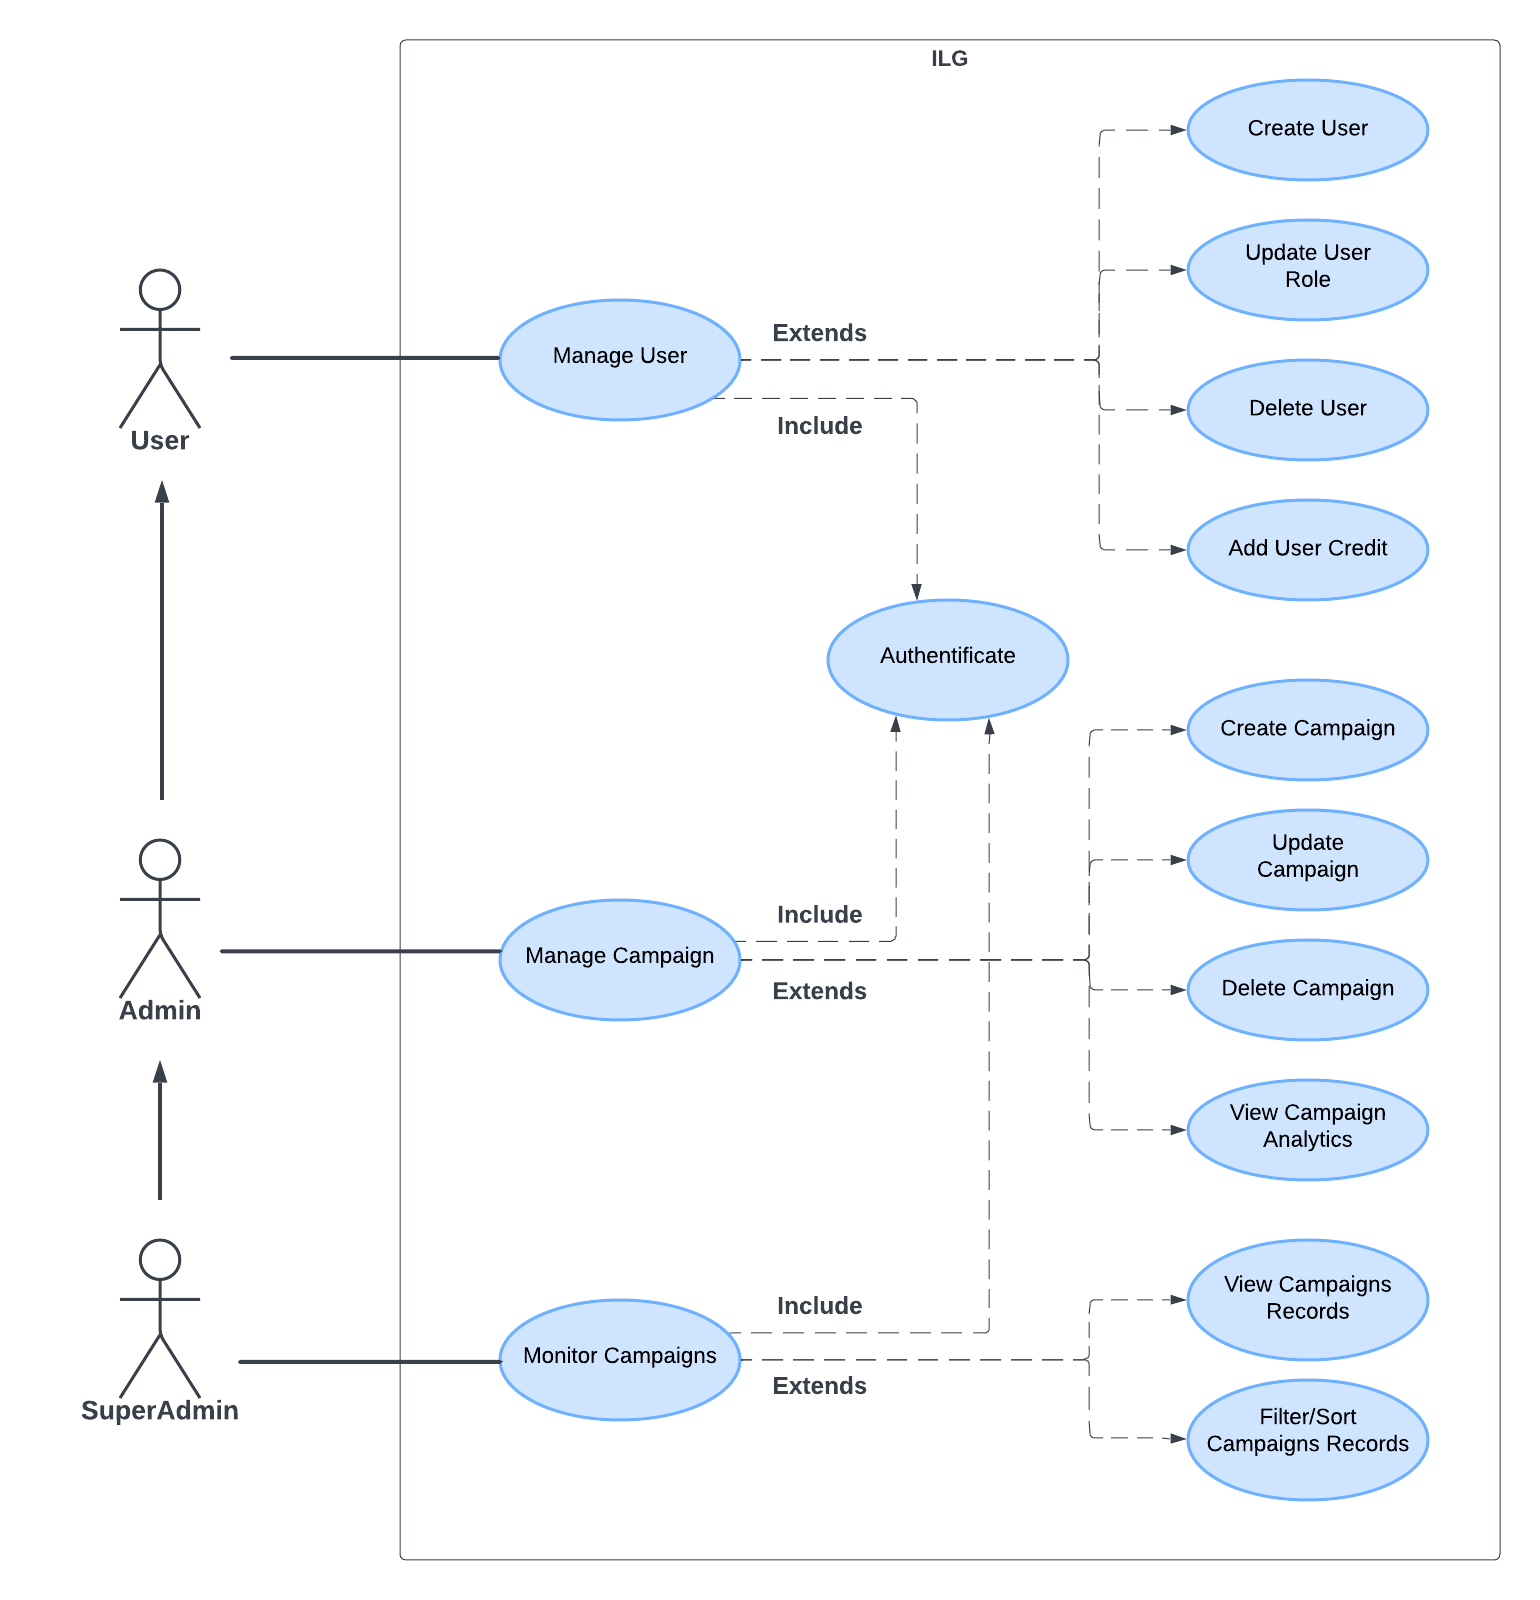
\includegraphics[width=\linewidth]{src/assets/diagrams/usecase.png}}
    \caption{Use case diagram for the frontend dashboard}
    \label{fig:use-case-diagram}
\end{figure}

\subsubsection{\underline{Use case textual description}}
Here is an example of the textual description of one of the use cases scenarios:
\begin{table}[H]
    \renewcommand{\arraystretch}{1.5}%
    \caption{Create Campaign's use case textual description}
    \centering
    \medskip
    \begin{tabularx}{1\textwidth} {
            | >{\hsize=0.5\hsize\linewidth=\hsize\centering\arraybackslash}X
            | >{\hsize=1.5\hsize\linewidth=\hsize\justifying\arraybackslash}X |}
        \hline
        \textbf {Use Case}         & \noindent Create Campaign                                                                                                              \\
        \hline
        \textbf {Actor}            & \noindent User.                                                                                                                        \\
        \hline
        \textbf {Pre-condition}    & \noindent Authenticated User.                                                                                                          \\
        \hline
        \textbf {Post-condition}   & \noindent Campaign Created.                                                                                                            \\
        \hline
        \textbf {Basic path}       & \noindent    \begin{enumerate}
            \item Navigate to campaign page.
            \item Click on the "create campaign" button.
            \item Fill in the needed information of the campaign in the popped modal form.
            \item Validate the form then submit.
        \end{enumerate}                                                                                                 \\
        \hline
        \textbf {Exceptional path} & \noindent On step 3, if the campaign sales navigator link is not valid, show "invalid campaign link" to the user and restart the step. \\
        \hline
    \end{tabularx}
\end{table}

% ----------------------- Conception ----------------------- %
\section{Conception}
In this section, we will dive deep into the conception and the logic behind the parts of the application:

% --------------- Non functional Requirements --------------- %
\section{Non-functional requirements}
Non functional requirements describe any specification that does not add direct business value but is nonetheless crucial for the good operation of a developed software.
For our app, what we should focus on is:
\begin{itemize}
    \item \textbf{Reliability and Availability:} The software should be available 24 hours a day and 7 days a week.
    \item \textbf{Security:} Clients should be able to safely login to the dashboard with a strong authentication system.
    \item \textbf{Maintainability and Recoverability:} We should respond to LinkedIn changes all the time as fast as possible.
    \item \textbf{Scalability:} This is the main reason we're migrating to a new architecture in the first place.
    \item \textbf{Documentation:} We should always document each and every step we make extensively so that new developers can onboard on the project in a fast and efficient way, which further emphasizes reliability.
\end{itemize}
% ----------------------------------- SECTIONS (^) ----------------------------------- %

\setcounter{secnumdepth}{0} % Set the section counter to 0 so next section is not counted in toc
% ----------------------- Conclusion ----------------------- %
\section{Conclusion}
In this chapter, we discussed our main objectives that we should meet during the course of our internship.
We also discuss the various layers and services of the application.
In what follows, we will discuss the realization part with heavy focus on DevOps and the actual implementation of the new architecture.
